\chapter{Versuchsaufbau}

\begin{figure}[h]
    \centering
    \includegraphics[width=.8\textwidth]{dokumente/hall-effekt_modul.jpg}
    \caption[Frontansicht Messmoduls]{Frontansicht des Moduls zur Messung des \textsc{Hall}-Effektes und der Leitfähigkeit der Probe \cite{PHYWESystemeGmbHundCo.KG.}}%
    \label{fig:messmodul}
\end{figure}

\begin{enumerate}
    \item Drehknopf für den Probenstrom $I_p$
    \item Digitalanzeige zur wahlweisen Anzeige von Probenstrom $I_p$
    \item Gewindebuchse zum Einschrauben des zugehörigen Haltestiels
    \item LED Anzeigenreihe für den Betriebszustand der Probenheizung und für die Anzeige des Probenstroms $I_p$ bzw. der Probentemperatur $T_p$ im LED-Display
    \item 4-mm-Sicherheitsbuchenpaar für den Abgriff der \textsc{Hall}-Spannung $U_H$
    \item Positionsdurchführung für eine tangentiale Magnetfeldsonde
    \item Druckschalter zur Auswahl der Anzeige von Probenstrom $I_p$ oder Probentemperatur $T_p$
    \item Drehknopf für die Fehlspannungskompensation der \textsc{Hall}-Spannung $U_H$
    \item Aufnahmeschacht für die Probenplatine mit Kontaktleiste
    \item 4-mm-Sicherheitsbuchsen für den Abgriff der Probenspannung $U_p$
\end{enumerate}

\begin{figure}[h]
    \centering
    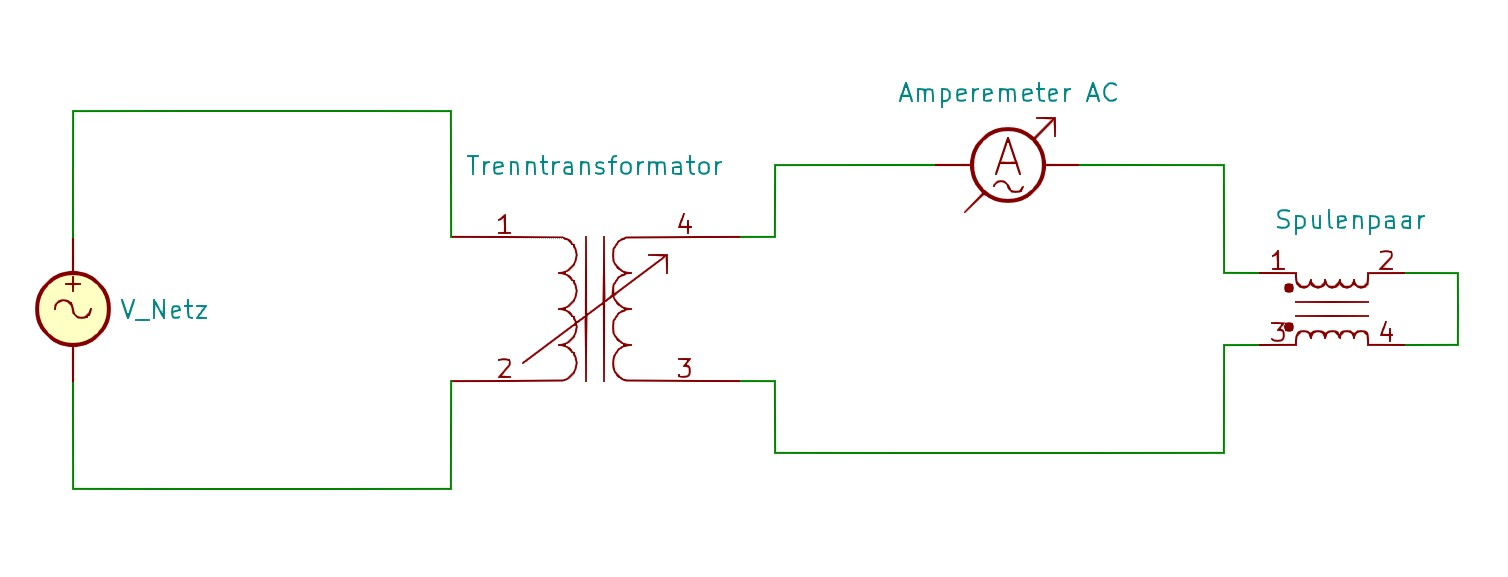
\includegraphics[width=.8\textwidth]{kicad/abbildungen/schematic_entmagnetisierung.jpg}
    \caption[Schaltskizze zur Entmagnetisierung]{Elektrischer Aufbau zur Entmagnetisierung der Spulen und des Eisenkerns.}%
    \label{fig:schematicEntmag}
\end{figure}

\begin{figure}[h]
    \centering
    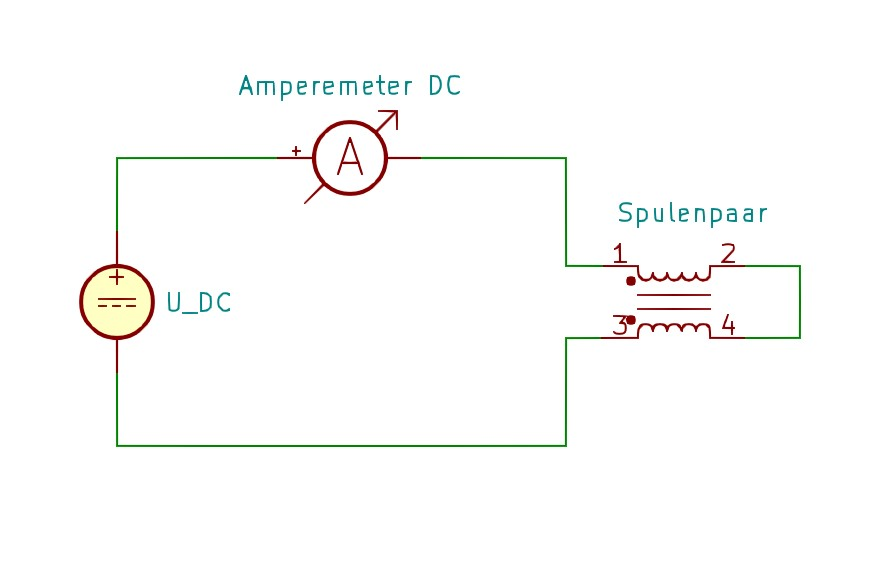
\includegraphics[width=.8\textwidth]{kicad/abbildungen/schematic_messung.jpg}
    \caption[Schaltskizze des Messaufbaus]{Elektrischer Aufbau zur Messung des Einflusses verschiedener Flussdichten auf die \textsc{Hall}-Spannung \(U_H\).}%
    \label{fig:schematicMessung}
\end{figure}


\begin{figure}[h]
    \centering
    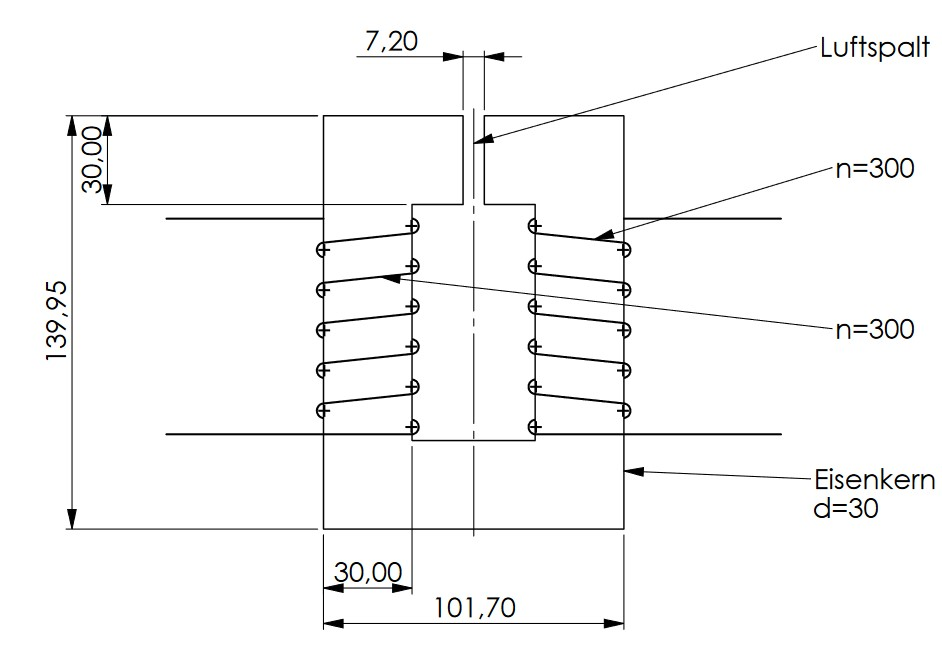
\includegraphics[width=.8\textwidth]{CAD/kern.jpg}
    \caption[Skizze des Spulenpaares mit Eiskenkern und Luftspalt]{Aufbau und Dimensionen des Eisenkerns mit Luftspalt und des Spulenpaares. Längeneinheiten in \si{\milli\metre}.}%
    \label{fig:zeichnungKern}
\end{figure}